\section{Functions}

\begin{frame}
    \frametitle{Definitions \& Properties}
    \framesubtitle{Basic definitions}
    Three essential factors of a function:
    \begin{itemize}
        \item Domain: $D$\\A set containing the action objects of correspondence rule.
        \item Correspondence Rule
        \item Range: $E$\\ A set of all images corresponding to all elements in the domain under a certain correspondence rule.
    \end{itemize}
    \begin{block}{Definition}
        A \textbf{function} $f$ is a rule that assigns to \alert{each element} $x$ in a set $D$ exactly one element, called $f(x)$, in a set $E$.
    \end{block}
    \begin{block}{The Vertical Line Test}
        A curve in the $xy$-plane is the graph of a function of $x$ \alert{iff} (if and only if) no vertical line intersects the curve more than once.
    \end{block}
\end{frame}

\begin{frame}
    \frametitle{Definitions \& Properties}
    \framesubtitle{Representation of Functions}
    There are four ways to represent a function:
    \begin{enumerate}
        \item Verbally (by a description in words)
        \item Numerically (by a table of values)
        \item Visually (by a graph)
        \item Algebraically (by an explicit formula)
    \end{enumerate}
\end{frame}

\begin{frame}
    \frametitle{Definitions \& Properties}
    \framesubtitle{Basic Properties}
    \begin{block}{Symmetry}
        \begin{itemize}
            \item Even function: $f(-x)=f(x)$
            \item Odd function: $f(-x)=-f(x)$
        \end{itemize}
        Tip: Give priority to whether the domain \textit{D} of the function is symmetrical.
    \end{block}
    \begin{block}{Increasing \& Decreasing property}
        A function $f$ is called (strictly) \textbf{increasing} on an interval $I$ if
        $$
            f\left(x_{1}\right)<f\left(x_{2}\right) \quad \text { whenever } x_{1}<x_{2} \text { in } I
        $$
        A function $f$ is called (strictly) \textbf{decreasing} on an interval $I$ if
        $$
            f\left(x_{1}\right)>f\left(x_{2}\right) \quad \text { whenever } x_{1}<x_{2} \text { in } I
        $$
    \end{block}
\end{frame}
\begin{frame}{Basic function types}
    \begin{block}{Linear function}
        The graph of the function is a line:
        \begin{center}
            $y=f(x)=mx+b$
        \end{center}
        $m$ is the slope of the line and $b$ is the y-intercept.
    \end{block}

    \begin{block}{Polynomials}
        A function $P$ is called a \textbf{polynomial} if
        \begin{center}
            $P(x)=\Sigma_{i=0}^n a_ix^i$
        \end{center}
        $a_i$ are \textbf{coefficients} and $n$ is the \textbf{degree} of the polynomial if $a_n\neq0$.
    \end{block}
    \begin{block}{Quadratic function}
        A polynomial of degree 2 is of the form $P(x)=ax^2+bx+c$ and is called a \textbf{quadratic function}.
    \end{block}

\end{frame}

\begin{frame}{Basic function types}
    \begin{block}{Power function}
        A function of the form $f(x)=x^a$ is called a \textbf{power function}, where $a$ is a constant. Consider an arbitary positive integer $n$:
        \begin{itemize}
            \item $a=n$:\\
                  \begin{center}
                      $y=x$: line \qquad $y=x^2$: parabola
                  \end{center}
            \item $a=\frac{1}{n}$: \textbf{root function}\\
            \item $a=-1$: \textbf{reciprocal function}
        \end{itemize}
    \end{block}
    \begin{block}{Ratio function}
        A \textbf{Ratio function} $f$ is a ratio of two polynomials:
        \begin{center}
            $f(x)=\frac{P(x)}{Q(x)}$
        \end{center}
        The domain consists of all values of $x$ such that $Q(x)\neq 0$.
    \end{block}
\end{frame}

\begin{frame}{Basic function types}
    \begin{block}{Trigonometric function}
        \begin{center}
            $\sin (x+2\pi)=\sin x\qquad \cos (x+2\pi)=\cos x\qquad $
            $\tan (x+\pi)=\tan x$
        \end{center}
    \end{block}
    \begin{block}{Exponential function}
        The \textbf{exponential functions} are the functions of the form $f(x) = a^x$, where the base a is a positive constant.
    \end{block}
    \begin{block}{Logarithmic function}
        The \textbf{logarithmic functions} $f(x) = \log_ax$, where the base $a$ is a positive constant and $a\neq 1$, are the inverse functions of the exponential functions.
    \end{block}
    Think about the question:\\
    What condition does $a$ meet when the exponential function increases in its domain? What about the logarithmic function?
\end{frame}

\begin{frame}{How to draw a function}
    \begin{itemize}
        \item You can simply trace the dots for simple functions.
        \item You may also try to use software:\\
              %\begin{center}
              https://www.geogebra.org\\
              https://www.desmos.com
              %\end{center}
    \end{itemize}
\end{frame}
\begin{frame}{Special Functions}
    \begin{block}{Dirichlet Function}

        $$
            1_{\mathbb{Q}}(x)= \begin{cases}1 & x \in \mathbb{Q} \\ 0 & x \notin \mathbb{Q}\end{cases}
        $$
    \end{block}
\end{frame}

\begin{frame}{Special Functions}
    \begin{block}{Impulse Function}

        $$
            \delta(t)= \begin{cases}\infty & t=0 \\ 0 & t \neq 0\end{cases}
        $$
    \end{block}
    \begin{block}{Step Function}
        $$
            H[n]= \begin{cases}0, & n<0 \\ 1, & n \geq 0\end{cases}
        $$
    \end{block}
    \begin{block}{Ramp Function}
        $$
            R(x):= \begin{cases}x, & x \geq 0 \\ 0, & x<0\end{cases}
        $$
    \end{block}
\end{frame}

\begin{frame}{Special Functions}
    \begin{block}{Hyperbolic Function}

        $$
            \sinh (x)=\frac{e^{x}-e^{-x}}{2}, \cosh (x)=\frac{e^{x}+e^{-x}}{2}, \tanh (x)=\frac{\sinh (x)}{\cosh (x)}
        $$
        %For more detail, see in textbook section $3.9$ and exercise.
    \end{block}
    \begin{block}{Inverse trigonometric function}

        $$
            \begin{aligned}
                 & \arcsin (x), \arccos (x), \arctan (x)                      \\
                 & \operatorname{arsinh}(x)=\ln \left(x+\sqrt{x^{2}+1}\right) \\ &\operatorname{arcosh}(x)=\ln \left(x+\sqrt{x^{2}-1}\right)\\ &\operatorname{artanh}(x)=\frac{1}{2} \ln \left(\frac{1+x}{1-x}\right)
            \end{aligned}
        $$
    \end{block}
\end{frame}
\begin{frame}{Function Transformation}
    \begin{block}{Vertical and Horizontal Shifts, suppose $c>0$}
        $y=f(x)+c$, shift the graph of $y=f(x)$ a distance $c$ units upward\\ $y=f(x)-c$, shift the graph of $y=f(x)$ a distance $c$ units downward\\ $y=f(x-c)$, shift the graph of $y=f(x)$ a distance $c$ units to the right\\ $y=f(x+c)$, shift the graph of $y=f(x)$ a distance $c$ units to the left\\
    \end{block}
    \begin{block}{Vertical and Horizontal Stretching and Reflecting, suppose $c>1$}
        $y=c f(x)$, stretch the graph of $y=f(x)$ vertically by a factor of $c$\\ $y=(1 / c) f(x)$, shrink the graph of $y=f(x)$ vertically by a factor of $c$\\
        $y=f(c x)$, shrink the graph of $y=f(x)$ horizontally by a factor of $c$\\ $y=f(x / c)$, stretch the graph of $y=f(x)$ horizontally by a factor of $c$\\
        $y=-f(x)$, reflect the graph of $y=f(x)$ about the $x$-axis\\ $y=f(-x)$, reflect the graph of $y=f(x)$ about the $y$-axis
    \end{block}
\end{frame}

\begin{frame}{Function Combination}
    \begin{block}{Definition}
        Given two functions $f$ and $g$, the \textbf{composite function} $f \circ g$ (also called the \textbf{composition} of $f$ and $g$ ) is defined by
        \begin{equation*}
            (f \circ g)(x)=f(g(x))
        \end{equation*}
    \end{block}
    \bigskip
    It is possible to take the composition of three or more functions. For instance, the composite function $f \circ g \circ h$ is found by first applying $h$, then $g$, and then $f$ as follows:
    $$
        (f \circ g \circ h)(x)=f(g(h(x)))
    $$
\end{frame}

\begin{frame}{Exercise 1}
    \textit{Skip it if you find the exercise quite simple.}\\
    \bigskip
    Find the domain of these functions:
    \begin{enumerate}
        \item $h(x)=\frac{1}{\sqrt[4]{x^{2}-5 x}}$\\
        \item $f(u)=\frac{u+1}{1+\frac{1}{u+1}}$\\
        \item $F(p)=\sqrt{2-\sqrt{p}}$
    \end{enumerate}
\end{frame}

\begin{frame}
    \frametitle{Exercise 1}
    \framesubtitle{Conclusions}
    \begin{block}{How to solve this kind of questions}
        \begin{itemize}
            \item The denominator in the fractional function cannot be zero
            \item The quantity in the even root formula cannot take a negative value, that is, it should be greater than or equal to zero
            \item The antilogarithm of the logarithm cannot be negative and zero, that is, it must take a positive value
            \item The domain of the function $y=\arcsin x, y=\arccos x$ is $-1 \leqslant x \leqslant 1$
            \item $y=\tan x$ , $x \neq k \pi+\pi / 2, y=\cot x$ , $x \neq k \pi$, $k$ is integer
        \end{itemize}
    \end{block}
\end{frame}

\begin{frame}{Exercise 2}
    \begin{block}{Prove or Disprove}
        \begin{itemize}
            \item If $f$ and $g$ are both even functions, is $f+g$ even? If $f$ and $g$ are both odd functions, is $f+g$ odd? What if $f$ is even and $g$ is odd? Justify your answers.
            \item If $f$ and $g$ are both even functions, is the product $f g$ even? If $f$ and $g$ are both odd functions, is $f g$ odd? What if $f$ is even and $g$ is odd? Justify your answers.
        \end{itemize}
    \end{block}
\end{frame}

\begin{frame}{Exercise 3}
    \begin{block}{Graph the functions step by step}
        (1)$y=1-2 \sqrt{x+3}$\\
        (2)$y=|\cos \pi x|$
    \end{block}
\end{frame}


\begin{frame}{Exercise 4}
    \begin{block}{Find the function (a) $f \circ g$, (b) $g \circ f$, (c) $f \circ f$, and (d) $g \circ g$ and their domains.}
        $f(x)=\frac{x}{1+x}, \quad g(x)=\sin 2 x$\\
    \end{block}
\end{frame}

\begin{frame}{Exercise 5}
    Find $f \circ g\circ h$:\\
    \begin{itemize}
        \item $f(x)=\tan x$
        \item $g(x)=\frac{x}{x-1}$
        \item $h(x)=\sqrt[3]{x}$
    \end{itemize}
    (It is unnecessary to find the domain of this composite function in this exercise!)
\end{frame}

\begin{frame}{Exercise 6}
    \begin{block}{Composite Function}
        \begin{enumerate}
            \item If $g(x)=2 x+1$ and $h(x)=4 x^{2}+4 x+7$, find a function $f$ such that $f \circ g=h$. \\(Think about what operations you would have to perform on the formula for $g$ to end up with the formula for $h$.)\\
            \item If $f(x)=3 x+5$ and $h(x)=3 x^{2}+3 x+2$, find a function $g$ such that $f \circ g=h$.\\
        \end{enumerate}
    \end{block}
\end{frame}

\begin{frame}{References}
    [1] Huang, Yucheng. VV156\_RC1\_updated.pdf. 2021.\\
    \bigskip
    [2] Cai, Runze. Chapter01.pdf. 2021.\\
    \bigskip
    [3] Zhou,Yishen.RC1. 2022.
\end{frame}

\begin{frame}{Exercise Answer 1-2}
    \begin{enumerate}
        \item $x^2-5x>0$ $\Rightarrow$ $x\in (-\infty,0)\cup (5,\infty)$
        \item $1+\frac{1}{u+1}\neq0,u+1\neq0$ $\Rightarrow$ $u\in (\infty,-2)\cup(-2,-1)\cup (-1,\infty)$
        \item $p\geq0,2-\sqrt{q}\geq0$ $\Rightarrow$ $p\in [0,4]$
    \end{enumerate}
    \vspace{1.5cm}
    \begin{itemize}
        \item Yes. Yes. Not necessarily.
        \item Yes. No.(fg is Even) fg is Odd.
    \end{itemize}
\end{frame}


\begin{frame}{Exercise Answer 3}
    \begin{center}
        (1)\\
        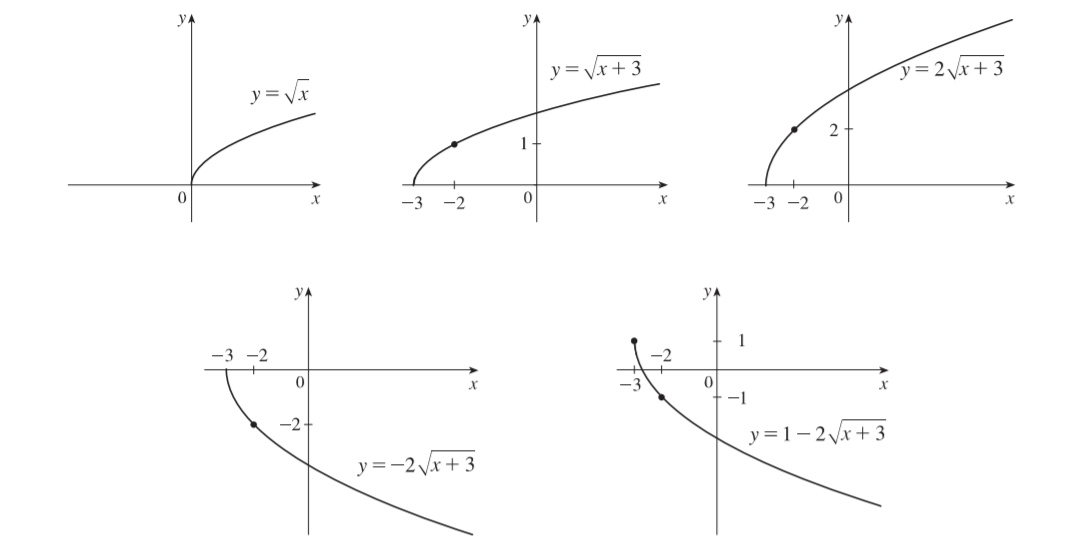
\includegraphics[width =8cm]{res/514.png}\\
        \vspace{1cm}
        (2)\\
        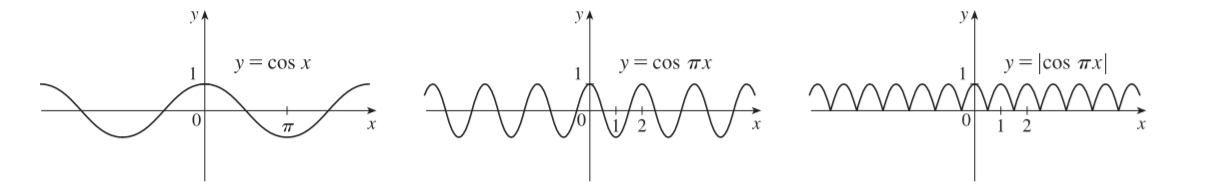
\includegraphics[width =8cm]{res/114.png}
    \end{center}
\end{frame}

\begin{frame}{Exercise Answer 4-5}
    (a) $f\circ g(x)=\frac{sin 2x}{1+sin 2x}$. Domain: $x\in\{x|x\neq k\pi-\frac{\pi}{4},k\in\mathbb{B}\}$\\
    (b) $g\circ f(x)=sin(\frac{2x}{1+x})$. Domain: $x\in (\infty,-1)\cup(-1,\infty)$\\
    (c) $f\circ f(x)=\frac{x}{1+2x}(x\neq-1)$. Domain:$x\in (\infty,-1)\cup(-1,-\frac{1}{2})\cup (-\frac{1}{2},\infty)$\\
    (d) $g\circ g(x)=sin(2sin(2x))$. Domain:$x\in\mathbb{R}$\\
    \vspace{1.5cm}
    $tan(\frac{\sqrt[3]{x}}{\sqrt[3]{x}-1})$
\end{frame}

\begin{frame}{Exercise Answer 6}
    \begin{enumerate}
        \item $x=\frac{g(x)-1}{2}$.\\
              Plug into h(x), $h(x)=4(\frac{g(x)-1}{2})^2+4(\frac{g(x)-1}{2})+7=g^2(x)+6$.\\
              Also, $h(x)=f(g(x))$.\\
              Therefore, $f(x)=x^2-6$
        \item $3g(x)+5=h(x)$, $g(x)=x^2+x-1$
    \end{enumerate}
\end{frame}